\documentclass{article}
\usepackage{natbib}
\usepackage{graphicx}
\usepackage{float}

\title{High-Performance Data Analysis on Janus using Apache Spark}
\author{Nick Vanderweit \\
        Ning Gao \\
        Anitha Ganesha \\
        Michael Kasper}

\begin{document}
\maketitle

\section{Introduction}
Over the past decade, there has been considerable interest in high-level
strategies for evaluating algorithms in parallel over large data sets.
Google's seminal MapReduce paper \citep{dean-mapreduce} describes such a
general strategy, which had already been in use at Google at the time of
publication, for building highly-scalable parallel applications out of small
serial functions. In general, phrasing data parallelism in terms of
higher-order functions on parallel data structures has proven fruitful
for many applications. In this paper, we evaluate Spark, a library
designed to address some of the shortcomings of MapReduce, on an existing
supercomputer.

In the MapReduce model, data is broken into \emph{splits} of a given size
before processing. These are stored on a distributed filesystem as key/value
pairs. The master node then distributes splits among the remaining workers.
Each of these workers runs a \emph{Map} on its split, computing for each
key/value pair $(k_1, v_1)$ another pair $(k_2, v_2)$. Each of these output
pairs is stored on the filesystem and the master is informed of their
locations. The master node proceeds by forwarding these intermediate pairs to the
\emph{Reduce} workers, which are responsible for combining the results for each
intermediate key.

A commonly-used example for this process is a distributed word count. First,
the input file (e.g. a large database dump containing posts on an Internet
forum) is broken into splits of a given size (say 64MB). The splits store
$(k, v)$ pairs such that each $v$ is a record (a post). The \emph{Map} task
is responsible for mapping each record to a set of (word, count) pairs,
which are written to the filesystem.

The next step is for a \emph{Reduce} worker to sort these records by key
and then sum together the values for each given key, and write out
a set of (word, count) records where the keys are now unique.

This simple example has interesting implications for MapReduce in general.
We can see that \emph{Map} tasks are highly-parallel, but \emph{Reduce}
introduces a serial bottleneck. In cases like parallel word count, where the
\emph{Reduce} is associative and commutative (i.e. forms a commutative
semigroup over the set of values), there is an additional opportunity for
parallelism. As such, MapReduce provides an additional task, called a
\emph{Combiner}, which assumes this structure and can be used to distill
the intermediate $(k, v)$ pairs before a \emph{Reduce}.

We can also see from this example a significant limitation of MapReduce: each
intermediate $(k, v)$ set is written to the distributed filesystem.  As such,
in order for MapReduce to be efficient, the individual tasks must be very
large.

However, some algorithms are not well-described by a simple map-and-then-reduce
pattern, and require multiple iterations.  If each iteration is small, the
algorithm's performance will be bottlenecked by this file I/O. For these
problems, another approach is needed.

Spark was designed at the UC Berkeley AMPLab to address these concerns using a
more flexible abstraction for distributed data \citep{zaharia}. Rather than
assuming that all intermediate data is stored on a filesystem, Spark uses
\emph{Resilient Distributed Datasets}, or RDDs, to represent data that is
stored on disk, cached in memory, or possibly has not been computed yet at all
\citep{zaharia_rdd}.  It is primarily targeted toward Scala, a statically-typed
functional language for the Java Virtual Machine.

\section{Overview}

\section{Evaluation}
% janus
    % overview
    % describe what spark test where
%%% DIRECTLY COPY-PASTED TEXT %%%
University of the University of Colorado's Top-
31 (June 2010) supercomputer system, Janus
    % specs (ref)
%%% DIRECTLY COPY-PASTED TEXT %%%
The final Janus computational
system consists of 1,368 nodes, each containing two six-
core Intel Xeon Westmere-EP chips at 2.8 GHz, for a total
of 2,736 processors and 16,416 cores with a theoretical
peak performance of 184 TFLOP/s. Each core has 2
GB of 1333 MHz DDR3 RAM for a total of 24 GB per
node and 32 TB of memory in the entire system. (REF)
% spark
    % reason for spark (diskless)
    % installation (default???)
    % version number (Spark 0.8.0, Scala 2.9.3)
% purpose of trials (speedup, efficiency, install on Janus)
    % find ideal configurations

\subsection{Testing}
% grep
    % overview
    % program source
    % grep complexity
    % file content
    % files sizes
    % node core counts
    % serial runtime
    % workers per node
% page rank
    % overview
    % ...

\subsection{Results}
% cores grep test
    % scale up, workers per node (graph)
    \begin{figure}[H]
        \centering
        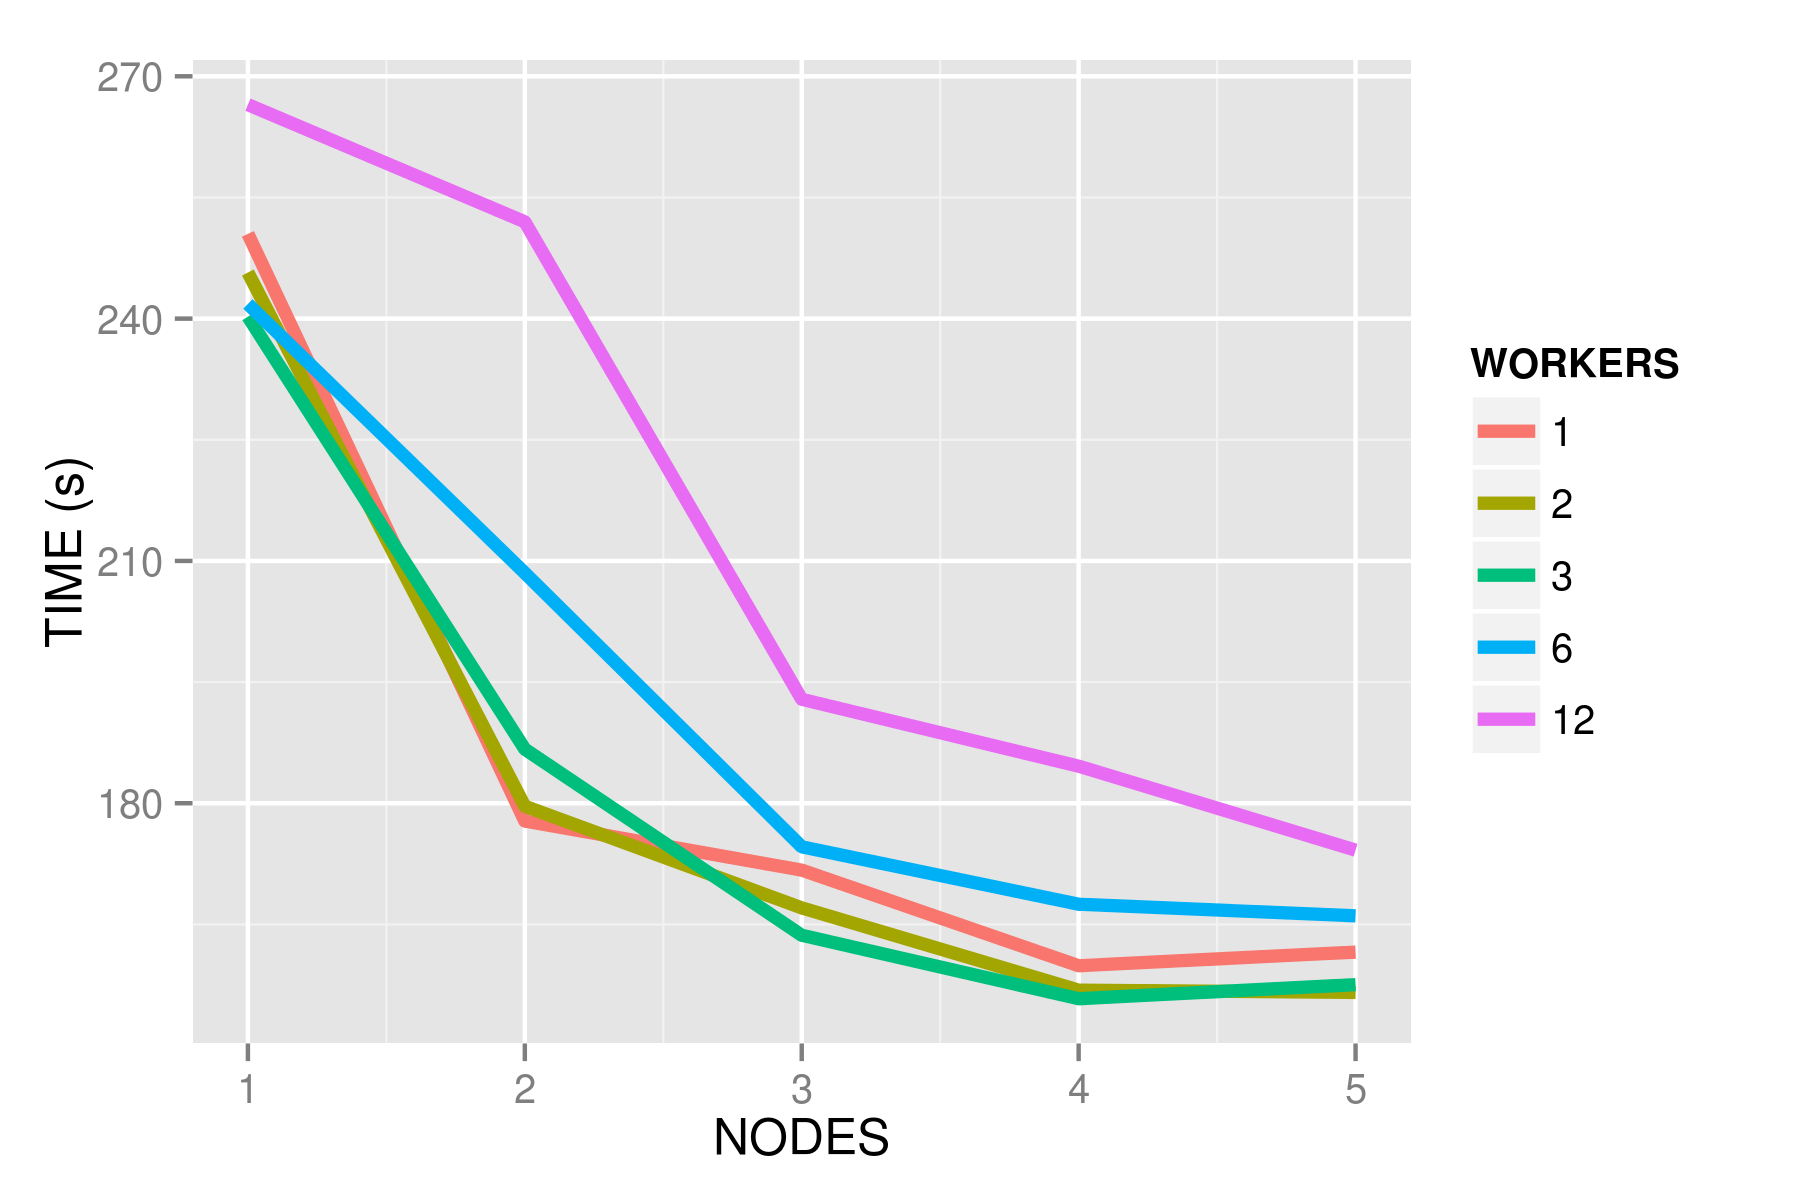
\includegraphics[width=90mm]{images/workerPerNodeTimes.png}
        \caption{Grep runtimes with different workers per node over 20GB file}
        \label{fig:workNodeTime}
    \end{figure}
    \begin{figure}[H]
        \centering
        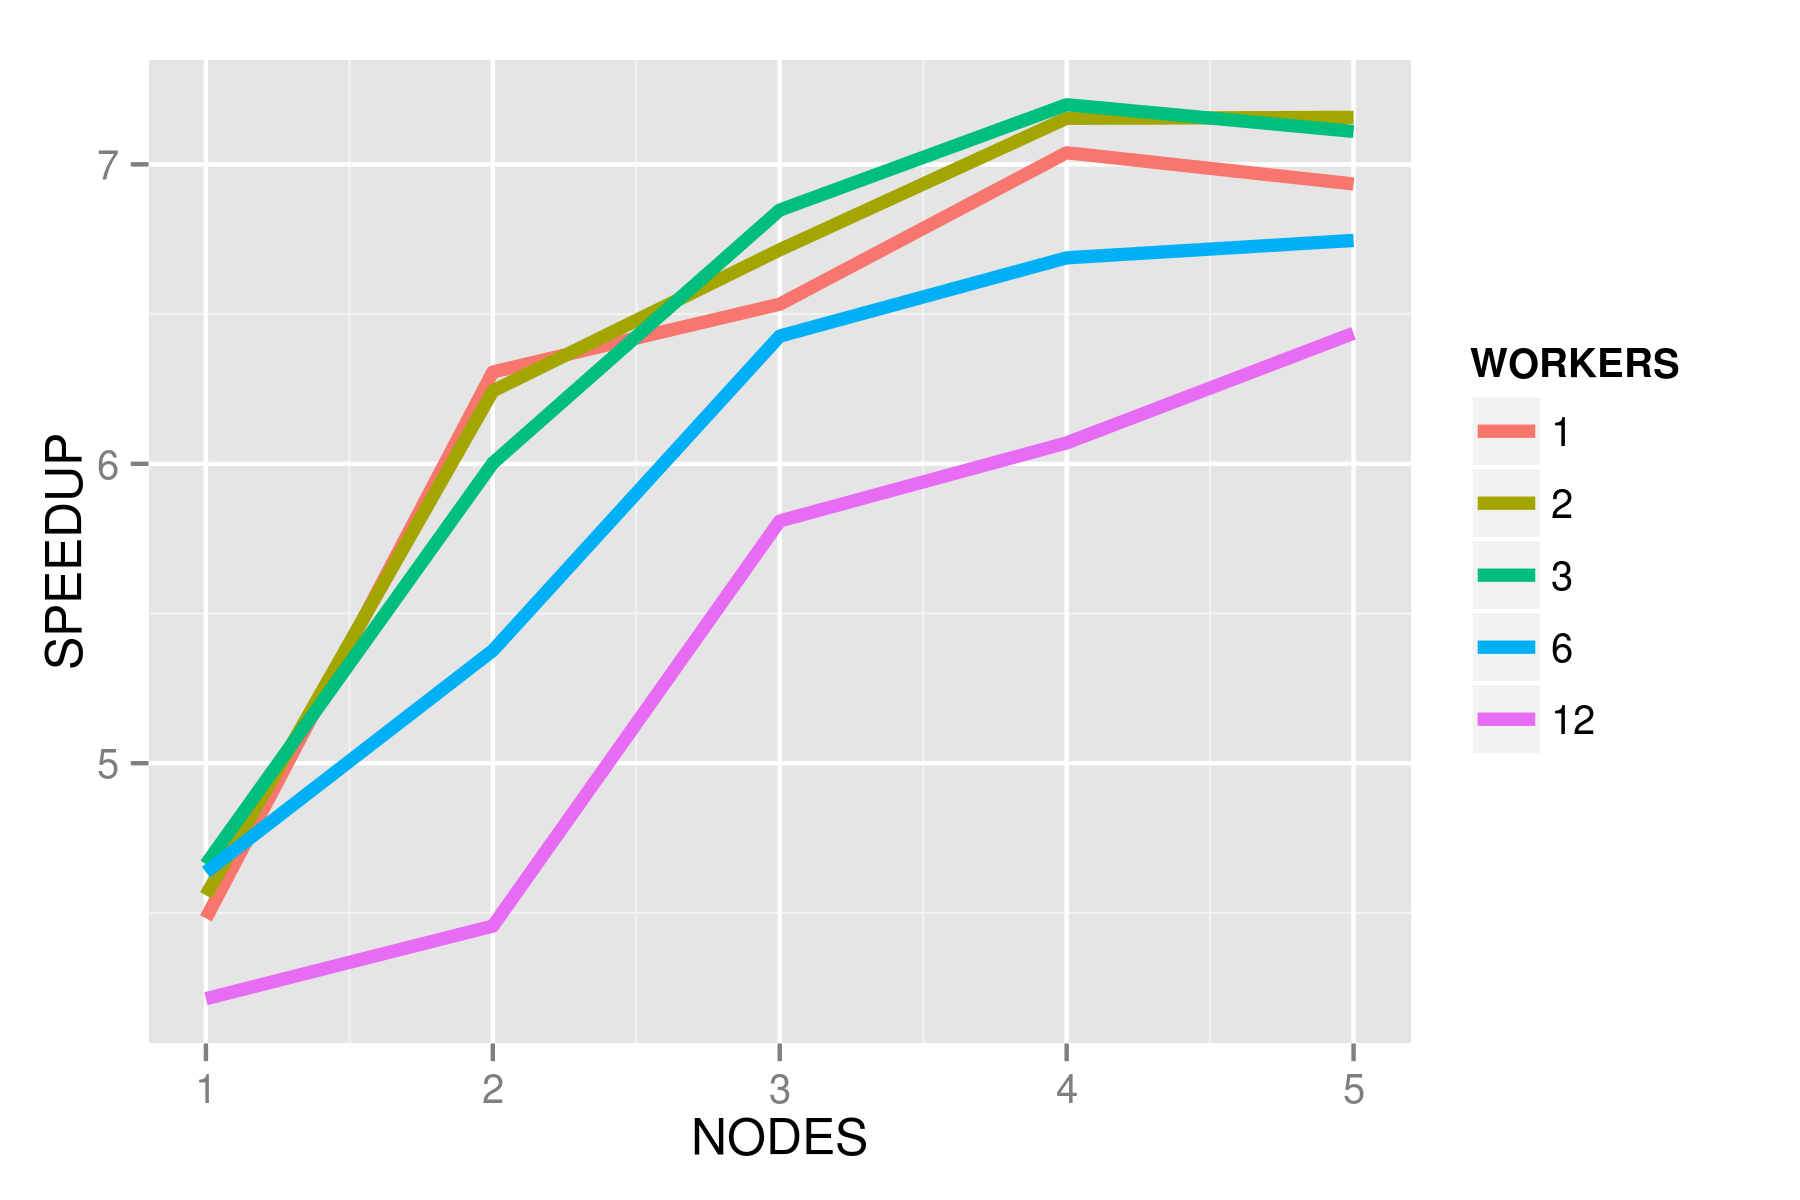
\includegraphics[width=90mm]{images/workerPerNodeSpeedup.png}
        \caption{Grep speedup with different workers per node over 20GB file}
    \end{figure}
    \begin{figure}[H]
        \centering
        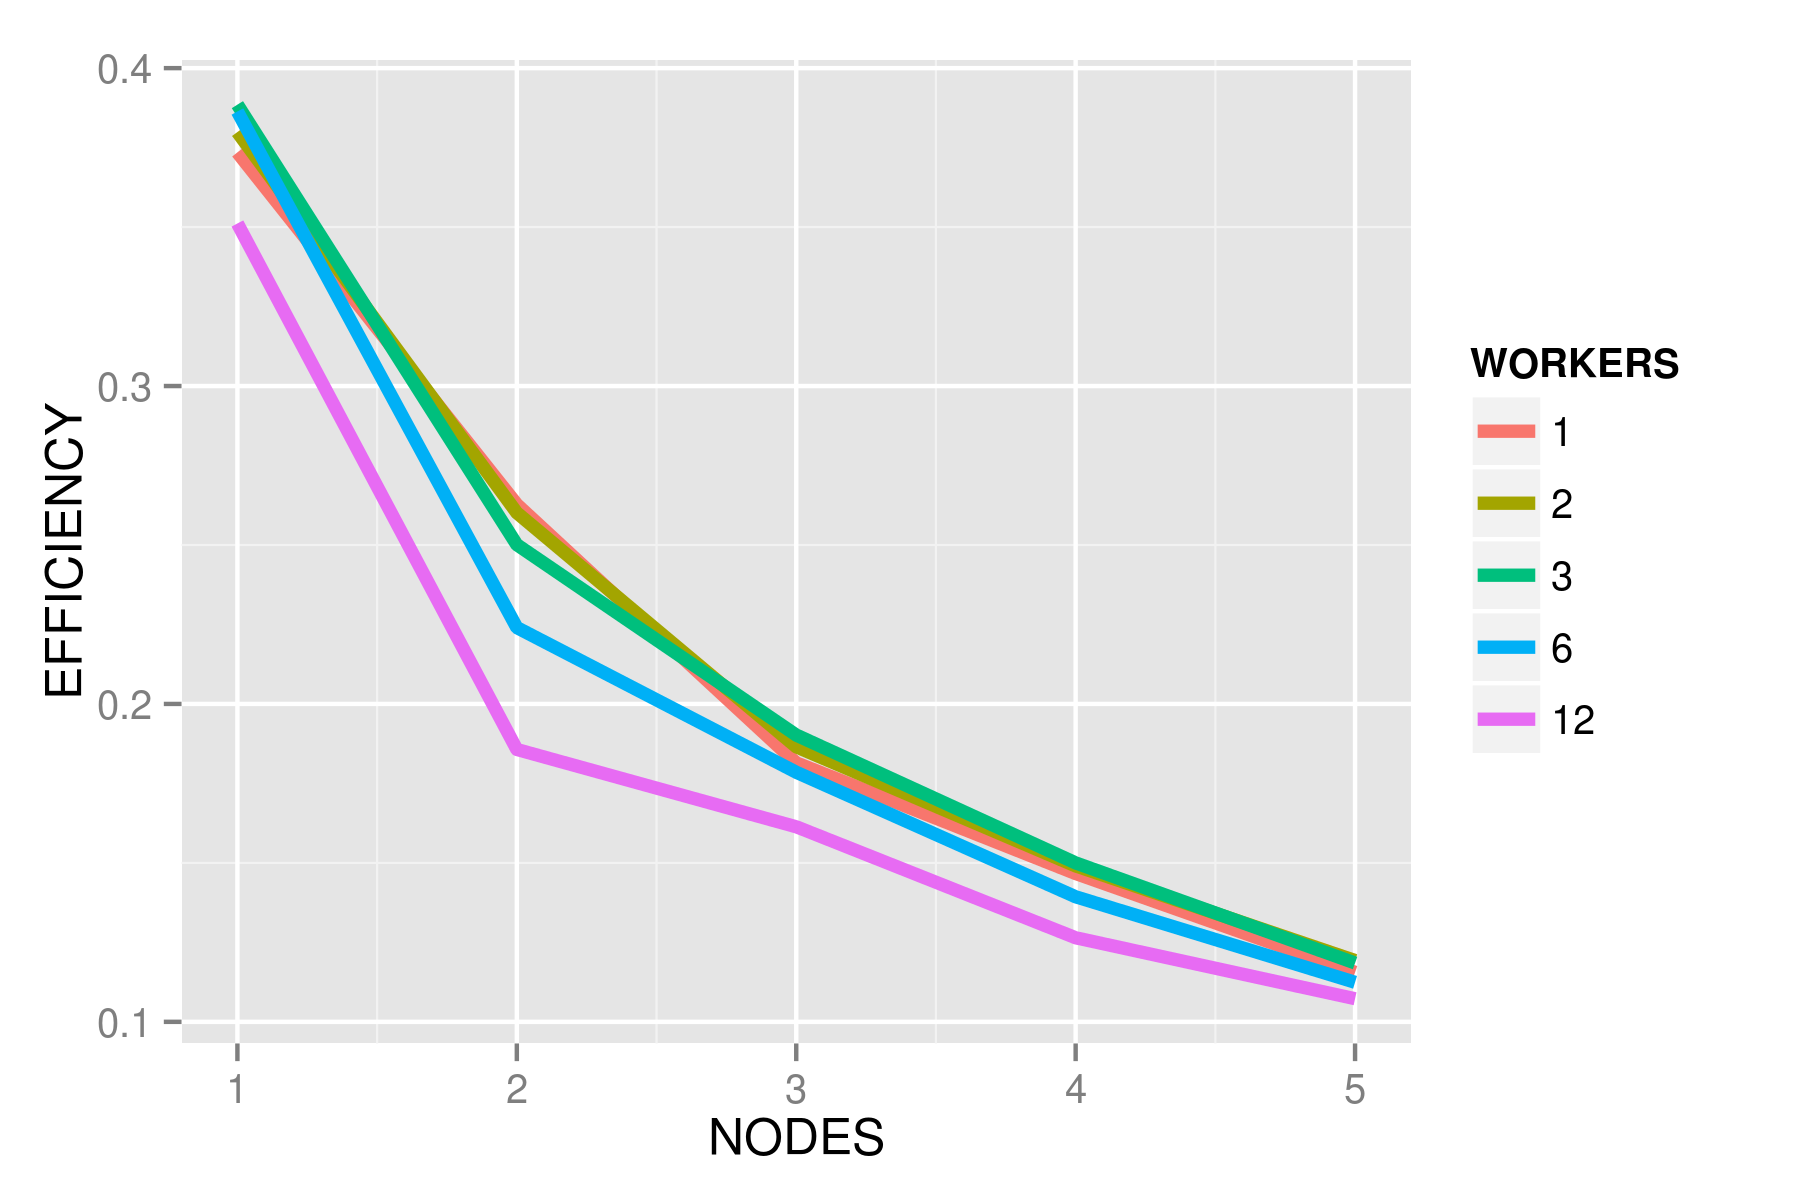
\includegraphics[width=90mm]{images/workerPerNodeEfficiency.png}
        \caption{Grep efficiency with different workers per node over 20GB file}
        \label{fig:workNodeEff}
    \end{figure}
    \begin{figure}[H]
        \centering
        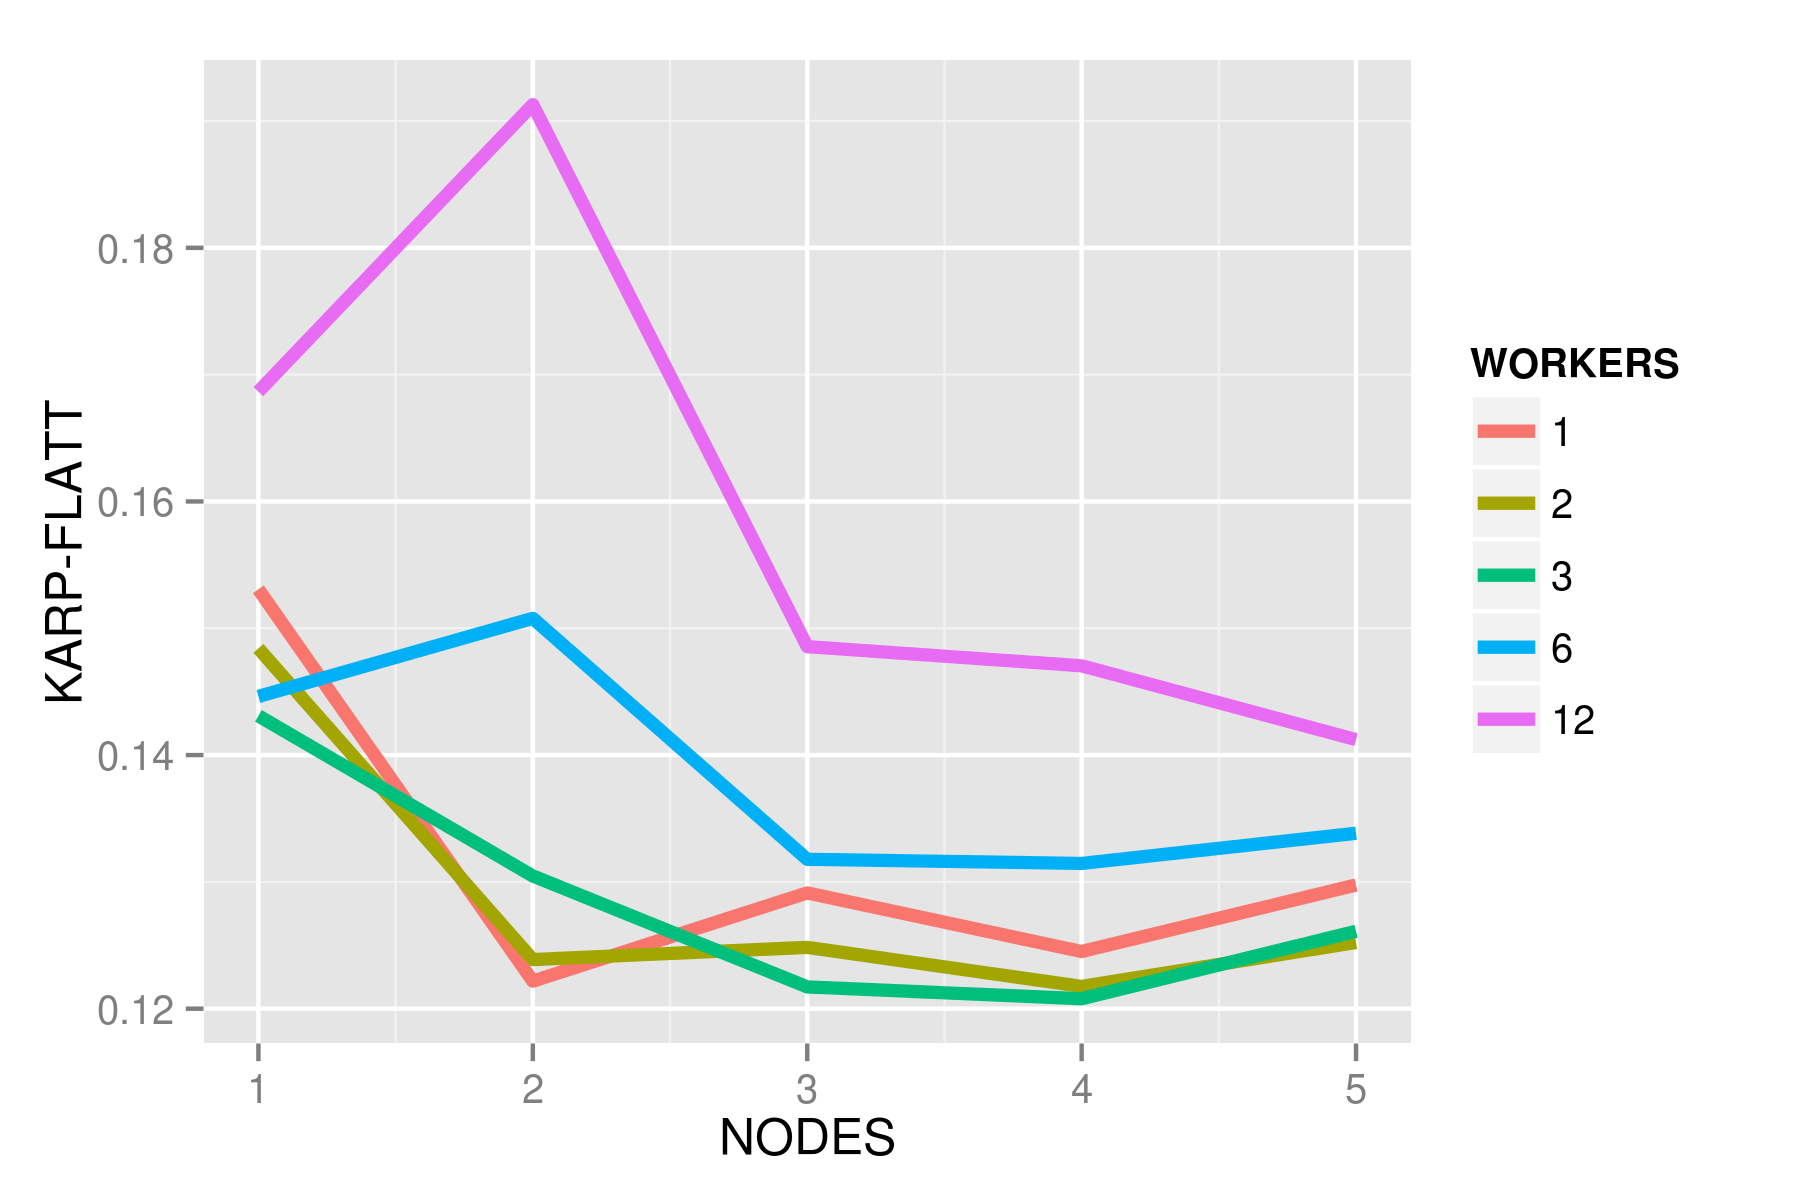
\includegraphics[width=90mm]{images/workerPerNodeKarpFlatt.png}
        \caption{Grep Karp-Flatt metric with different workers per node over
                20GB file}
        \label{fig:workNodeKF}
    \end{figure}
        % stays relative constant, serial is the issue
% large grep test
    % serial run time (graph)
    \begin{figure}[H]
        \centering
        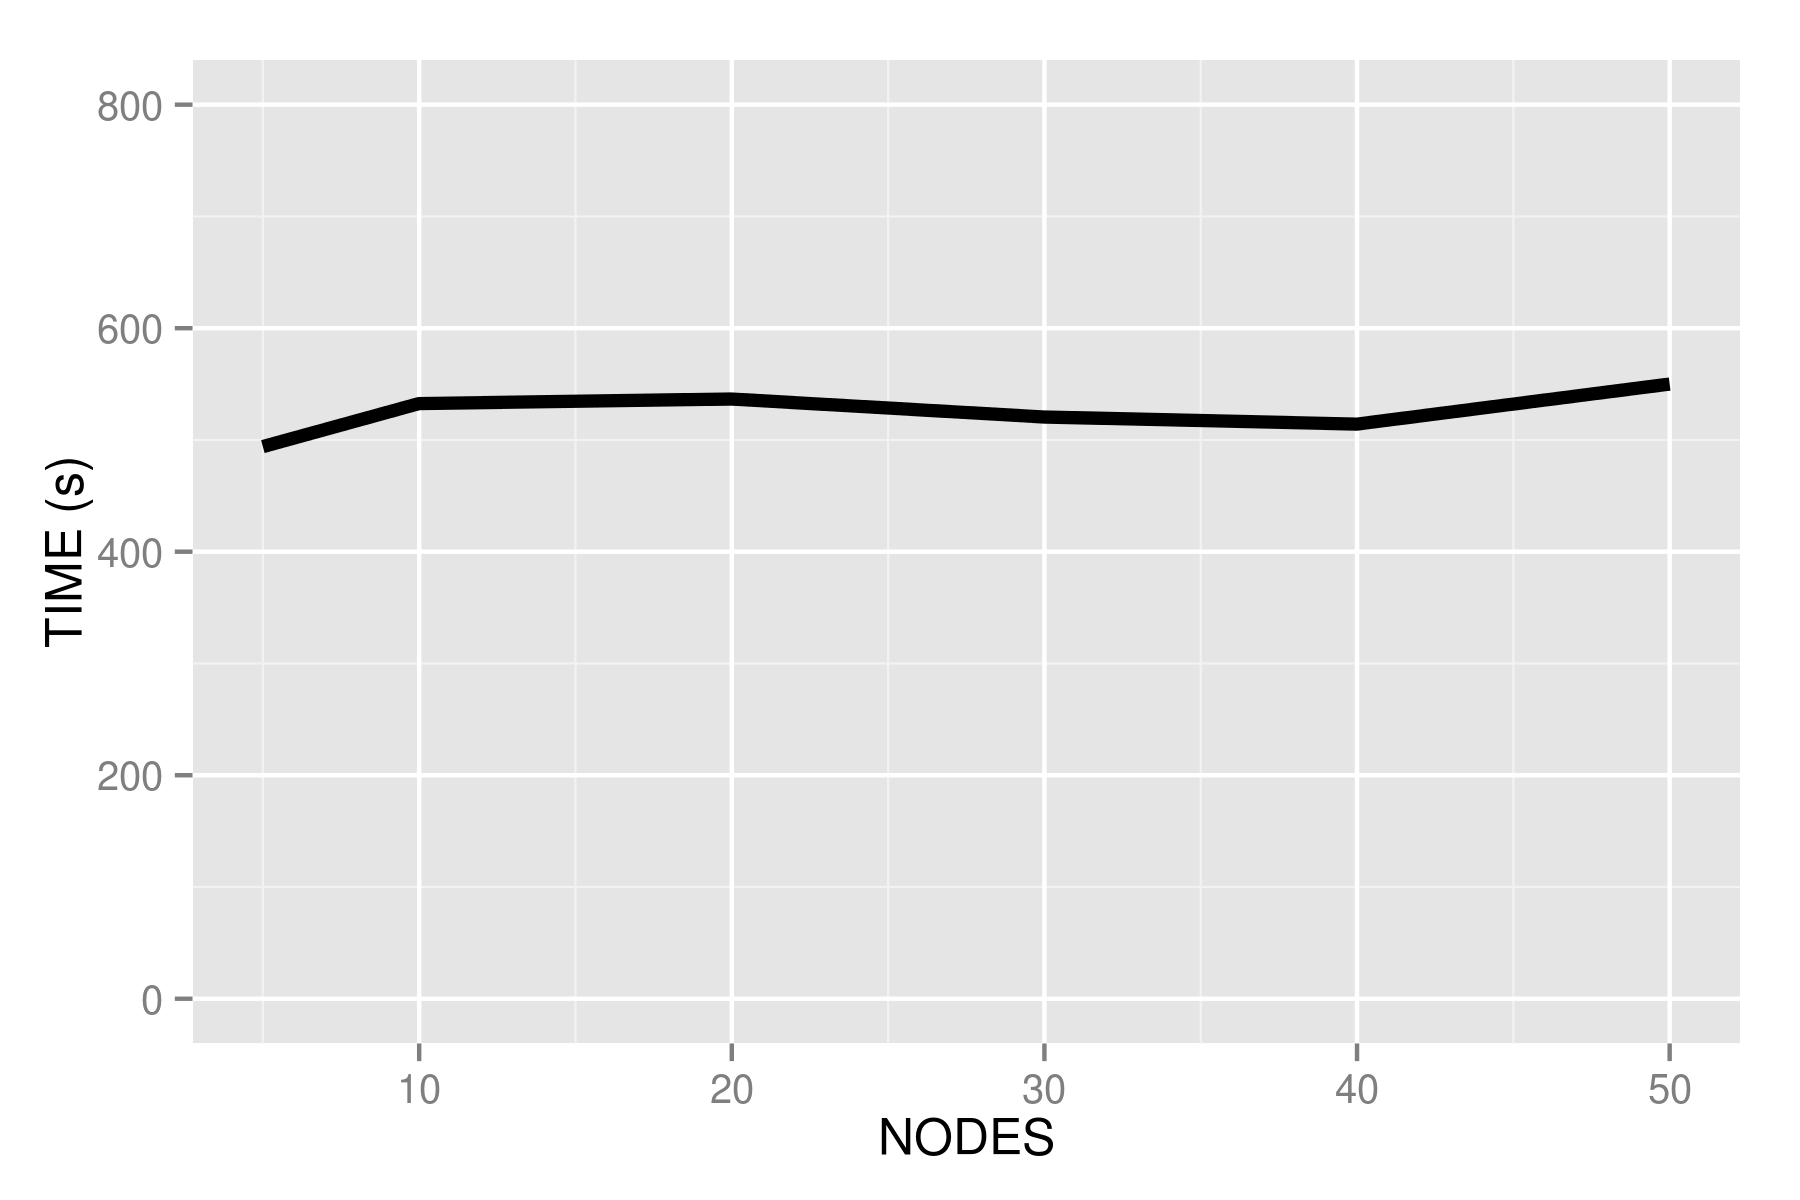
\includegraphics[width=90mm]{images/bigDataTimes.png}
        \caption{Average grep runtimes over 100GB file}
        \label{fig:bigTime}
        % stays relative constant, serial is the issue
    \end{figure}
% pagerank test 1
% pagerank test 2
% ...

\section{Discussion}
% small grep test
    % ideal balance between speedup and efficiency
% cores grep test
    % ideal number of workers per core
    % close enough not to matter
    % don't use 6-12
% large grep test
    % ideal workers per problem size
    % follow up test with delay
    % take away on IO
% pagerank test 1
% pagerank test 2
% ...

% workings and master comm of spark protocol

\section{Conclusion}

\bibliography{paper}
\bibliographystyle{plain}

\end{document}
